\begin{frame}{Discutons d'une ville}
  En groupes de 3 ou 4, lisez cette description de Dakar et discutez de la question ci-dessous.
  \vspace{0.25cm}
  \begin{columns}
    \small
    \column{0.65\textwidth}
      Dakar est un centre administratif et commercial du Sénégal et dispose du plus grand port d'Afrique.
      Cette ville est la capitale politique, économique et culturelle du pays.
      Elle comprend le quartier historique de la Médina et le célèbre musée Théodore Monod exposant des œuvres d'art africain.
      Elle est également réputée pour sa vie nocturne, centrée sur la musique Mbalax.
      Sa population est cosmopolite et comprend toutes les ethnies du pays malgré le fait que les Wolofs soient les plus représentés.
      Il y a plusieurs sites touristiques et plusieurs stations balnéaires où on peut nager.
    \column{0.35\textwidth}
      \begin{center}
        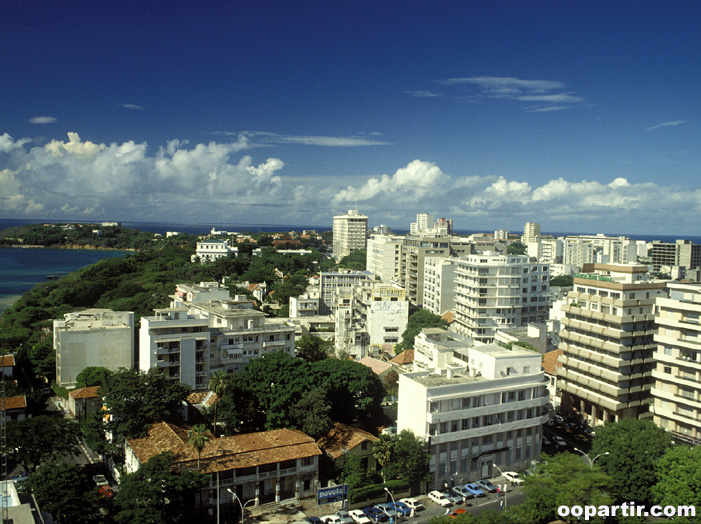
\includegraphics[scale=0.16]{dakar.jpg}
      \end{center}
      Est-ce que vous voudriez visiter ou habiter Dakar?
      Pourquoi ou pourquoi pas?
  \end{columns}
\end{frame}